\documentclass[MS, xcolor=dvipsnames]{wfuthesis}
\usepackage{mathtools,amsthm,amssymb,mathrsfs}
\usepackage{graphicx}
\usepackage{xcolor}
\usepackage{enumitem}
\usepackage{pdfpages}

% \usepackage[backend=biber]{biblatex}
% \addbibresource{bibliography.bib}
\usepackage[pdfpagelabels,draft,implicit=false]{hyperref}
\urlstyle{same}
% \usepackage{soul}
% \usepackage{float}
% \usepackage{enumerate}
% \usepackage{multicol}
% \usepackage{tikz}
% \usetikzlibrary{matrix,arrows}
% \usepackage[all]{xy}
% \usepackage{tikz-cd}
% \tikzcdset{every arrow/.append style = -{Latex[width=4pt,length=10pt]}}
\usepackage[defaultmono]{droidsansmono}
\usepackage{listings}
% \lstset{basicstyle=\xpt\droidsansmono}
% \usepackage{fontspec}
% \usepackage{setspace}
% \setmainfont{Times New Roman}
% \usepackage{derivative}
% \usepackage{fancyvrb}
% \renewcommand{\theFancyVerbLine}{\textsuperscript{\arabic{FancyVerbLine}}}
% \usepackage{multirow}
% \usepackage{dsfont}
\usepackage{indentfirst}
% \usepackage{blindtext}
\usepackage{lipsum}

\definecolor{codegreen}{rgb}{0,0.6,0}
\definecolor{codegray}{rgb}{0.5,0.5,0.5}
\definecolor{codepurple}{rgb}{0.58,0,0.82}
\definecolor{backcolour}{rgb}{0.95,0.95,0.92}

\lstset{escapechar=\&,
        basicstyle=\xpt\droidsansmono,
        breaklines=true,
        showstringspaces=false,
        backgroundcolor=\color{backcolour},   
        commentstyle=\color{codegreen},
        keywordstyle=\color{blue},
        stringstyle=\color{codepurple}}

% \DeclarePairedDelimiter{\ceil}{\lceil}{\rceil}
% \DeclarePairedDelimiter{\floor}{\lfloor}{\rfloor}
% \def\bA{\mathbb{A}}
% \def\cB{\mathcal{B}}
\def\bC{\mathbb{C}}
\def\bF{\mathbb{F}}
% \def\bH{\mathbb{H}}
% \def\bI{\mathbb{I}}
% \def\cL{\mathcal{L}}
% \def\cM{\mathcal{M}}
\def\bN{\mathbb{N}}
\def\cP{\mathcal{P}}
\def\bQ{\mathbb{Q}}
\def\bR{\mathbb{R}}
% \def\cT{\mathcal{T}}
% \def\cU{\mathcal{U}}
% \def\bV{\mathbb{V}}
\def\bZ{\mathbb{Z}}
% \def\bk{\bk}
\def\sbs{\subseteq}
\def\sps{\supseteq}

% \newcommand{\upperset}[2]{\:
% \underset{
%   \text{\raisebox{1.2ex}{\smash{\scalebox{0.8}{$#1$}}}}
% }{
%   \text{\raisebox{0.2ex}{\smash{$#2$}}}
% }
% \:}
% \def\opset{\upperset{\text{\tiny{open}}} \subset}
% \def\clset{\upperset{\text{\tiny{closed}}} \subset}

% \DeclareMathOperator{\Aut}{Aut}
% \DeclareMathOperator{\Dim}{Dim}
% \DeclareMathOperator{\ev}{ev}
% \DeclareMathOperator{\GL}{GL}
% \DeclareMathOperator{\Hom}{Hom}
\DeclareMathOperator{\id}{id}
\DeclareMathOperator{\im}{im}
% \DeclareMathOperator{\Mat}{Mat}
% \DeclareMathOperator{\nullsp}{null}
% \DeclareMathOperator{\range}{range}
% \DeclareMathOperator{\SL}{SL}
\DeclareMathOperator{\Span}{span}
\DeclareMathOperator{\lcm}{lcm}
\newcommand{\LT}{\ensuremath{\text{\sc lt}}}
\newcommand{\LM}{\ensuremath{\text{\sc lm}}}
\newcommand{\LC}{\ensuremath{\text{\sc lc}}}
\DeclareMathOperator{\multideg}{multideg}
\def\and{\text{ and }}

\newtheorem{theorem}{Theorem}
\newtheorem{lemma}[theorem]{Lemma}
\newtheorem{observation}[theorem]{Observation}
\newtheorem{proposition}[theorem]{Proposition}
\newtheorem{corollary}[theorem]{Corollary}
\theoremstyle{definition}
\newtheorem{definition}[theorem]{Definition}
\newtheorem{example}[theorem]{Example}

% \def\e{\epsilon}
% \def\d{\delta}
% \def\p{\varphi}

\begin{document}
\title{A Functional Computer Algebra System for Polynomials}
\author{Thomas Meek}
\department{Mathematics}

\advisor{W. Frank Moore, Ph.D.}
\chairperson{Ellen Kirkman, Ph.D.}
\member{William Turkett, Ph.D.}

\date{April, 2023}

\maketitle

\clearpage

\acknowledgements 

\lipsum[1]

\tableofcontents

\abstract

The \lstinline{polynomial-algorithms} package is a computer algebra system written in Haskell. This package implements a Polynomial type for use in several algorithms including a recursive version of Buchberger's algorithm for finding the reduced Gr\"obner basis of a polynomial ideal. As it is written in Haskell, the \lstinline{polynomial-algorithms} package naturally uses a purely functional design philosophy. We will contrast this with imperative approaches using more traditional languages. 

\chapters

\chapter{Introduction}
The theory of polynomials is a well-studied field of mathematics, rich with results which provide tools for mathematicians in various areas. Polynomial functions are among the simplest continuous functions to work with analytically or algebraically. Computationally, they are unquestionably the most important class of functions. It is then imperative to have a robust collection of software that can assist the mathematicians who study them. Many tools currently exist for this purpose, from dedicated high-level languages like Macaulay2 and Singular to libraries for general purpose languages like SageMath and SimPy. These software collections are referred to as \textit{computer algebra systems} or CAS's and while most have capabilities beyond polynomial manipulation, it is this feature that is the focus here. \par 
The implementation of these tools varies greatly. The Macaulay2 engine is written in C++\cite{M2} while SageMath is built with Python\cite{sagemath}, which in turn often calls C. Their respective interfaces often use a mixture of procedural, object-oriented, functional, and declarative design. This certainly makes sense in the case of SageMath as Python itself hybridizes these approaches. If a CAS is a package for a general purpose language like Python, it should obey the design principles of that language. For dedicated CAS's like Macaulay2 though, this design choice bears consideration. There is a tendency in modern languages to incorporate features which favor a variety of paradigms. The popularity of hybrid languages like Python and JavaScript has encouraged most newer languages like Rust and Go to follow in their footsteps. There are good reasons for this, however there are also benefits to sticking to a single paradigm. \par 
It is true that these paradigms are more a philosophical way of approaching software design than a well-defined feature of a language and given that, no language can be said to be strictly single paradigm. It is clear however that certain languages lend themselves to being more compatible with one paradigm than others. For example, Java is generally seen as a paragon of object-oriented programming. Every module contains exactly one class (with potentially many subclasses). Even the drivers are classes and must be instantiated before any program can be executed. One can use Java in a functional way, but doing so defeats the purpose of using Java. This is in contrast to a language like Python where it is difficult to escape the use of objects and classes, but higher order functions like folds and maps are used frequently, as are list comprehensions and other hallmarks of functional programming. At the same time, most programmers' first experience with Python is in writing plain procedural scripts. The freedom offered by such a language enables one to chose the most appropriate approach to the current task, but in doing so, it takes away the cohesiveness and predictability of a more \textit{pure} language like Java. \par 
Similarly to the way Java is considered a paragon of the object-oriented school, Haskell is often one of the first two languages people think of when one mentions functional programming, with the other of course being Lisp. The functional style offers many advantages over a procedural or object-oriented approach as evidenced in how much modern languages have borrowed from Haskell. Rust's type system strongly resembles that of Haskell\cite{poss2014} and modern JavaScript libraries like React  leverage functional programming more than any other paradigm. \par 
Haskell and the functional programming style are particularly well-suited to mathematics. The notion of a `function' in procedural programming is a bit of a misnomer. Mathematically, a function $f$ is a domain $X$, a codomain $Y$, and some subset of $X \times Y$ called the graph of $f$. What is the domain of the \lstinline{print()} function in Python? What is its codomain? What is its graph? These inconsistencies vanish in Haskell. A Haskell function \textit{is} a mathematical function. For this reason, mathematicians often regard the functional paradigm as the natural choice for mathematical software. What better way to determine the injectivity of a function than with a function whose injectivity can be determined?! \par 
It is in this spirit that the \lstinline{polynomial-algorithms} package was written. Taking advantage of the benefits offered by Haskell (as well as a few language extensions), this package offers a Polynomial type that is itself built on Monomial and Coefficient types. Several algorithms, most notably a modified version of Buchberger's algorithm to find a reduced Gr\"obner basis for a list of polynomials, are featured in this software. In addition, its scalability and modularity should provide mathematicians with an invaluable tool when analyzing polynomials. 

\chapter{Mathematical Background}
One thing that sets functional programming apart from imperative paradigms is its reliance on mathematics. Writing algorithms or any sufficiently complex code will always require some familiarity with mathematics, and the best and most efficient code is often written by programmers competent in mathematical reasoning. However, this quality is even more important when working in a language like Haskell. This fact may be seen just by reading documentation. A good technical writer will always write to their audience. If one is writing a UDP server in Java, it may be assumed that anyone maintaining that server will be familiar with terms like \textit{port}, \textit{buffer}, or \textit{packet}, so they may appear frequently in documentation. If one is writing an operating system in C, terms like \textit{fork} and \textit{process ID} are ubiquitous enough to appear in documentation without explanation. However, one is unlikely to encounter mentions of algebraic ring theory in the documentation for such projects. When using Haskell, this is quite common\cite{Prelude}. \par 
It is therefore imperative (pun intended) for a prospective Haskeller\footnote{The term \textit{Haskeller} refers to a regular user of Haskell.} to have a working knowledge of several areas of mathematics not usually necessary for writing programs in a procedural or object-oriented style. This is doubly important when using Haskell to write a CAS. The fact that the recommended backgrounds for the problem domain and the solution domain coincide is further evidence that Haskell is indeed a good fit for such a task. \par 
As any software engineer will tell you, having a firm understanding of mathematical logic can be helpful in writing and debugging code. Boolean algebra is essential for the standard control flow mechanisms used in all languages. De Morgan's laws and other properties of first order logic can assist in cleaning up messy functions. It is well-known that a familiarity with combinatorics and graph theory can be helpful for those writing abstract data types or analyzing networks, and linear algebra and multivariate calculus are essential for working with 3D graphics. However, abstract algebra and category theory are rarely covered in the standard curriculum for a computer science degree. \par 
When using Haskell, a working knowledge of algebraic group theory and ring theory, while not strictly necessary, can provide useful insight into why certain typeclasses and functions behave the way they do. When writing a CAS, this recommendation is upgraded to a strict requirement. Even more central in the design of Haskell and other functionally minded languages is the presence of the ever-intimidating category theory. Even by theoretical mathematicians, this subject is often referred to as \textit{abstract nonsense}\cite{Saunders97}. Having a reputation as as being among the most abstruse of mathematical topics, the mere fact that something as concrete and useful as writing software could employ such a concept is itself remarkable. \par 
Using such a mathematically inclined language to implement a CAS is clearly an endeavour that requires a thorough understanding of the mathematics at play. Of particular importance is the theory of polynomials. 

\section{Polynomials}
Polynomials in a single variable with real coefficients are a familiar object of study, not only to professional mathematicians, but to anyone who has taken a high school math class. They are easy to understand and work with. Finding their roots, taking their derivatives, and analyzing their graphs are among the easier tasks a mathematician will attempt. We even estimate arbitrary analytic functions as polynomials via Taylor's theorem. Many of the algorithms that form the backbone of low-level software are based on this idea. It should come as no surprise then that generalizing these familiar objects is a popular practice. Using fields other than $\bR$ is a natural first step. In fact, when using an algebraically closed field like $\bC$, polynomials behave even more nicely than they did over $\bR$ as we don't have to wonder how many roots a degree $n$ polynomial may have; the answer is always $n$ (up to multiplicity). \par 
The next natural generalization is to allow for multiple (though still finitely many) variables. This generalization does introduce some complexity. For one thing, the idea of ordering the terms, which was taken for granted in the single variable case, now becomes a nontrivial discussion. The tools from multivariate calculus can be helpful in understanding the analytic nature of multivariate polynomials, while an introductory course in abstract algebra or algebraic geometry often addresses the more algebraic concerns by introducing term orders, algorithms, and the relationship between the ideals containing these objects and the affine varieties they generate. 

\subsection{Monomials}
There are two competing ways to view a polynomial. The first is as a function from some ring into itself. It is this view that is usually encountered first, and for most analytic purposes, this is sufficient. The other way is as a formal linear combination of indeterminates. This is the view that we prefer in this discussion. These indeterminates comprise a free monoid\footnote{Recall that a monoid is a set with an associative binary operation and an identity element. Being free means there are no unforced relationships between elements. For example, $x \ne y^n$ for any $n$.}, and (at least for now) we may assume the monoidal operation to be commutative. We use the term \textit{monomial} when referring to elements of a free monoid in the context of polynomials. \par 
In this view, the phrase \textit{polynomial in n variables} really means a linear combination of monomials drawn from a free monoid with $n$ distinct generators. Each generator is called a variable. When dealing with polynomials in a single variable, we usually use the symbol $x$ to refer to the generator of this monoid. So the polynomial $f$ defined as 
\[ f(x) = x^2-8x+15 \]
is a formal linear combination of the monomials $x^2$, $x$, and $1$ taken from the free monoid $\langle x \rangle$ with weights $1$,$-8$, and $15$. In the case of a three variable polynomial, the monoid used is generated by three elements. Here, there are two competing notational conventions. The first is to denote the generators as $x$, $y$, and $z$. The second is to denote the generators as $x_1$, $x_2$, and $x_3$. The former is often more readable, but the latter more easily generalizes to $n$ variables. \par 
This viewpoint of polynomials as a formal combination of monomials rather than a function may be summed up in the following few definitions courtesy of Cox, Little and O'Shea\cite{Cox2015}: 
\begin{definition}
  A \textbf{monomial} in $x_1,\dots,x_n$ is a product of the form 
  \[ x_1^{\alpha_1} \cdot x_2^{\alpha_2} \cdots x_n^{\alpha_n}, \]
  where all of the exponents $\alpha_1,\dots,\alpha_n$ are nonnegative integers. The \textbf{total degree} of this monomial is the sum $\alpha_1 + \dots + \alpha_n$.
\end{definition}
We can simplify the notation for monomials as follows: let $\alpha = (\alpha_1,\dots,\alpha_n)$ be an $n$-tuple of nonnegative integers. Then we set
\[ x^\alpha = x_1^{\alpha_1} \cdot x_2^{\alpha_2} \cdots x_n^{\alpha_n}. \]
When $\alpha=(0,\dots,0)$, note that $x^\alpha=1$. We also let $|\alpha| = \alpha_1 + \dots + \alpha_n$ denote the total degree of the monomial $x^\alpha$.
\begin{definition}
  A \textbf{polynomial} $f$ in $x_1,\dots,x_n$ with coefficients in a field $k$ is a finite linear combination (with coefficients in $k$) of monomials. We will write a polynomial $f$ in the form
  \[ f = \sum_\alpha a_\alpha x^\alpha,\quad a_\alpha \in k, \]
  where the sum is over a finite number of $n$-tuples $\alpha = (\alpha_1,\dots,\alpha_n)$. The set of all polynomials in $x_1,\dots,x_n$ with coefficients in $k$ is denoted $k[x_1,\dots,x_n]$. 
\end{definition}
\begin{definition}
  Let $f = \sum_\alpha a_\alpha x^\alpha$ be a polynomial in $k[x_1,\dots,x_n]$. 
  \begin{enumerate}[label=(\roman*)]
    \item We call $a_\alpha$ the \textbf{coefficient} of the monomial $x^\alpha$. 
    \item If $a_\alpha\ne0$, then we call $a_\alpha x^\alpha$ a \textbf{term} of $f$. 
    \item The \textbf{total degree} of $f \ne 0$, denoted $\deg(f)$, is the maximum $|\alpha|$ such that the coefficient $a_\alpha$ is nonzero. The total degree of the zero polynomial is undefined.
  \end{enumerate}
\end{definition}
One observation is that the set $k[x_1,\dots,x_n]$ forms a ring under the standard polynomial addition and multiplication operations. In the case where $n=1$, the ring $k[x]$ contains the familiar polynomials in a single variable. An important question that often arises when working with polynomials in more than one variable is how to define the leading term. Given a nonzero polynomial $f \in k[x]$, let
\[ f = c_0x^m + c_1x^{m-1} + \dots + c_m, \]
where $c_i \in k$ and $c_0 \ne 0$ (thus $\deg(f)=m$). Then we say that $c_0x^m$ is the \textbf{leading term} of $f$ and write $\LT(f)=c_0x^m$. The leading term of a polynomial is a surprisingly essential characteristic. For example, when executing single variable polynomial long division, the first step is to make sure the polynomial is expressed with its leading term first, and at each subsequent step, that must remain the case; but what about when there are multiple variables? Given the polynomial $g \in k[x,y,z]$ defined as 
\[ g = xy^2z^3 + x^5 + x^3y^2z, \]
what is the leading term of $g$? We will have to be careful about how we define the leading term in this case, as there is not just one obvious way. \par 
This leads us to a discussion of \textit{monomial orderings}. There are uncountably many ways to order the monomials in a free monoid, but the majority of them will not be compatible with polynomial multiplication in the way we would like. The orderings that we may use must satisfy a few special properties, espoused in the following definition\cite{Cox2015}:
\begin{definition}
  A \textbf{monomial ordering} on $k[x_1,\dots,x_n]$ is a relation $>$ on the set of monomials $x^\alpha$, $\alpha \in \bZ_{\ge0}^n$ satisfying:
  \begin{enumerate}[label=(\roman*)]
    \item $>$ is a total ordering\footnote{Recall $>$ is a total ordering if for all $\alpha,\beta$ exactly one of $x^\alpha > x^\beta$, $x^\alpha = x^\beta$, or $x^\beta > x^\alpha$ is true.}. 
    \item If $x^\alpha > x^\beta$ and $\gamma \in \bZ_{\ge0}^n$, then $x^\alpha x^\gamma > x^\beta x^\gamma$. 
    \item $>$ is a well-ordering. 
  \end{enumerate}
\end{definition}
It turns out that the third condition above is equivalent to two other statements that are easier to work with. 
\begin{theorem}
  Let $X$ be a commutative free monoid and suppose the first two conditions in the definition above are satisfied. The the following are equivalent: 
  \begin{enumerate}
    \item $>$ is a well-ordering on $X$. 
    \item Every strictly decreasing sequence in $X$ eventually terminates. 
    \item $x^\alpha>0$ for all $\alpha \in \bZ_{\ge0}^n$. 
  \end{enumerate}
\end{theorem}
For a proof of this theorem, see Cox, Little and O'Shea\cite{Cox2015}. This allows us to show that certain algorithms terminate by showing that some term strictly decreases at each step of the algorithm. \par 
Now that we have a well-defined way to order monomials, we are ready to define a few more terms.
\begin{definition}
  Let $f = \sum_\alpha a_\alpha x^\alpha$ be a nonzero polynomial in $k[x_1,\dots,x_n]$ and let $>$ be a monomial order.
  \begin{enumerate}[label=(\roman*)]
    \item The \textbf{multidegree} of $f$ is 
    \[ \multideg(f) = \max(\alpha \in \bZ_{\ge0}^n \mid a_\alpha \ne 0) \]
    (the maximum is taken with respect to $>$).
    \item The \textbf{leading coefficient} of $f$ is
    \[ \LC(f) = a_{\multideg(f)} \in k. \]
    \item The \textbf{leading monomial} of $f$ is
    \[ \LM(f) = x^{\multideg(f)}. \]
    \item The \textbf{leading term} of $f$ is
    \[ \LT(f) = \LC(f) \cdot \LM(f). \]
  \end{enumerate}
\end{definition}
There are many monomial orderings that are used frequently in research, however we will limit our attention to three specific examples. The first such example is perhaps the most intuitive. 
\begin{definition}[\bf Lexicographic Order]
  Let $\alpha = (\alpha_1, \dots, \alpha_n)$ and $\beta = (\beta_1,\dots,\beta_n)$ be in $\bZ_{\ge0}^n$. We say $x^\alpha >_{Lex} x^\beta$ if the leftmost nonzero entry of the vector difference $\alpha - \beta \in \bZ^n$ is positive. 
\end{definition}
The Lexicographic order is the order used in a dictionary. We begin with an ordering of the variables. The greater monomial is the one with the larger exponent in the first variable. If those exponents are the same, we instead calculate the Lexicographic order without the highest variable. In our previous example, $g = xy^2z^3 + x^5 + x^3y^2z$, we see that the lead term under the Lexicographic order where $x>y>z$ is $\LT(g)=x^5$. By convention, when denoting variables with subscripts, we take $x_1 > x_2 > x_3 > \dots$. \par 
Our next monomial ordering is built out of the Lexicographic order. 
\begin{definition}[\bf Graded Lex Order]
  Let $\alpha,\beta \in \bZ_{\ge0}^n$. We say $x^\alpha >_{GLex} x^\beta$ if $|\alpha| > |\beta|$ or $|\alpha|=|\beta|$ and $x^\alpha >_{Lex} x^\beta$. 
\end{definition}
This means that the Graded Lex order first orders by total degree, but breaks ties with the Lexicographic order. In our running example using the Graded Lex order, we see that $\LT(g)=x^3y^2z$. \par 
Our third and final monomial ordering is less intuitive than the previous two.
\begin{definition}[\bf Graded Reverse Lex Order]
  Let $\alpha,\beta \in \bZ_{\ge0}^n$. We say $x^\alpha >_{GRevLex} x^\beta$ if $|\alpha| > |\beta|$ or $|\alpha|=|\beta|$ and the rightmost nonzero entry of $\alpha - \beta \in \bZ^n$ is negative. 
\end{definition}
Here, we are still ordering first by total degree, but we break ties in a manner that is in a way the reverse of Lexicographic order. Using the Graded Reverse Lex order, the lead term of $g$ is $xy^2z^3$. As unintuitive as the Graded Reverse Lex order may seem, it turns out that this ordering is often the most efficient in many algorithms, including some we will explore here. 

\subsection{Ideals}
In general, when $R$ is a commutative ring, a subring $I$ (not necessarily with identity) is an ideal if $ra \in I$ for all $r \in R$ and $a \in I$. For the polynomial ring $k[x_1,\dots,x_n]$ this means that an ideal is a nonempty subset closed under subtraction which absorbs polynomials by multiplication. For example, let $S \sbs k[x]$ be the set of polynomials with no constant or linear terms, so that $0 \in S$ and for any nonzero $f \in S$, the lowest degree term of $f$ has degree at least two. Then $S$ is easily seen to be an ideal of $k[x]$. In fact, $S$ is what is known as a \textit{principle ideal} because $S$ is \textit{generated} by a single polynomial, namely the polynomial $x^2$. This means that any polynomial in $S$ may be formed by multiplying $x^2$ by some polynomial in $k[x]$. More generally, an ideal $I \in k[x_1,\dots,x_n]$ is said to be generated by a set $B$ of polynomials if every $f \in I$ may be expressed as $f = b_1f_1 + \dots + b_tf_t$ for some $b_1,\dots,b_t \in B$ and some $f_1,\dots,f_t \in k[x_1,\dots,x_n]$. In this case, we write $I = \langle B \rangle$. In our example above, we would write $S = \langle x^2 \rangle$. It turns out that \textit{every} ideal in $k[x]$ is generated by a single polynomial, making this ring quite important in algebra and number theory. When dealing with multiple variables, we have no such luck. There is no single polynomial that generates the ideal $\langle x,y \rangle \in k[x,y,z]$. However, it is true that every polynomial ideal is generated by \textit{some} set since an ideal will generate itself. What is more impressive and not quite as obvious is the fact that every polynomial ideal is generated by some \textit{finite} set. This result was first proved by David Hilbert in 1890 and is known as \textit{Hilbert's Basis Theorem}\cite{Hilbert90}. \par 
Combining our notion of the leading term of a polynomial with ideals in a polynomial ring leads us to the following definition.
\begin{definition}
  Let $I \sbs k[x_1,\dots,x_n]$ be an ideal other than $\{0\}$, and fix a monomial ordering on $k[x_1,\dots,x_n]$. Then: 
  \begin{enumerate}[label=(\roman*)]
    \item We denote by $\LT(I)$ the set of leading terms of nonzero elements of $I$. Thus,
    \[ \LT(I) = \{ cx^\alpha \mid \text{ there exists } f \in I \setminus \{0\} \text{ with } \LT(f) = cx^\alpha \}. \]
    \item We denote by $\langle \LT(I) \rangle$ the ideal generated by the elements of $\LT(I)$. 
  \end{enumerate}
\end{definition}
If $I \sbs k[x_1,\dots,x_n]$ is an ideal then by Hilbert's Basis Theorem, there is some finite set of polynomials $\{ b_1,\dots,b_t \} \sbs k[x_1,\dots,x_n]$ such that $I = \langle b_1,\dots,b_t \rangle$. Since $b_1,\dots,b_t \in I$, it is clear that $\langle \LT(b_1), \dots, \LT(b_t) \rangle \sbs \langle \LT(I) \rangle$. However, this containment may be proper. Only in a very special case do we achieve equality of these two sets.

\subsection{Gr\"obner bases}
We mentioned polynomial long division before when making the case for why a monomial ordering is necessary. Another challenge when working with multiple variables is that, even when we have the requisite ordering to preform long division, the quotient and remainder may depend on the order of the dividends. When dividing $f$ by the ordered list $(g_1,g_2,g_3)$, we may get a different result from when dividing $f$ by the ordered list $(g_2,g_3,g_1)$. While the quotient is unfortunately doomed to this fate, there is a way we may guarantee the uniqueness of at least the remainder. It turns out this uniqueness is crucial for many of the theorems and algorithms that mathematicians rely on. \par 
\begin{definition}
  Fix a monomial order on the polynomial ring $k[x_1,\dots,x_n]$. A finite subset $G = \{ g_1,\dots,g_t \}$ of an ideal $I \sbs k[x_1,\dots,x_n]$ different from $\{0\}$ is said to be a \emph{Gr\"obner basis} if
  \[ \langle \LT(g_1), \dots, \LT(g_t) \rangle = \langle \LT(I) \rangle. \]
  Using the convention that $\langle \emptyset \rangle = {0}$, we define the empty set $\emptyset$ to be the Gr\"obner basis of the zero ideal $\{0\}$.
\end{definition}
Another way to state this definition is that the set $G = \{ g_1,\dots,g_t \}$ is a Gr\"obner basis for $I$ if the leading term of any element of $I$ is divisible by one of the $\LT(g_i)$. As one would expect, a Gr\"obner basis is indeed a basis for the ideal $I$ in the definition above and it can be shown that every ideal has a Gr\"obner basis. This is lucky because much of modern polynomial theory and algebraic geometry depends on the existence of such a basis. This is partly because the Gr\"obner basis is the set we needed to guarantee uniqueness of the remainder in the division algorithm. \par 
Another feature of Gr\"obner bases is a solution to the so called \emph{ideal membership problem}. For a proof of the following theorem, see \cite{Cox2015}.
\begin{theorem}
  Let $G = \{ g_1,\dots,g_t \}$ be a Gr\"obner basis for an ideal $I \sbs k[x_1,\dots,x_n]$ and let $f \in k[x_1,\dots,x_n]$. Then $f \in I$ if and only if the remainder on division of $f$ by $G$ is zero. 
\end{theorem}
The remainder is sometimes called the \emph{normal form} of $f$. We will use the following notation for the remainder.
\begin{definition}
  We will write $\overline f^{F}$ for the remainder on division of $f$ by the ordered $s$-tuple $F = (f_1,\dots,f_s)$. If $F$ is a Gr\"obner basis for $\langle f_1,\dots,f_s \rangle$, then we can regard $F$ as a set  (without any particular order). 
\end{definition}
One application of the division algorithm is Buchberger's algorithm for finding a Gr\"obner basis for the ideal $\langle f_1,\dots,f_t \rangle$. The idea behind this algorithm is to start with a list $(f_1,\dots,f_t)$, determine all polynomials in $\langle f_1,\dots,f_t \rangle$ that may have a lead term that isn't divisible by any of the $\LT(f_i)$, and add to the list the ones that aren't. To find a polynomial with lead term that isn't divisible by any of the $\LT(f_i)$, we need to construct a polynomial in our ideal that has a potentially different lead term from the generators. We do this by calculating \emph{$S$-polynomials}. The way we check if the $S$-polynomial is in our ideal already is via the division algorithm. 
\begin{definition}
  Let $f,g \in k[x_1,\dots,x_n]$ be nonzero polynomials. 
  \begin{itemize}
    \item If $\multideg(f) = \alpha$ and $\multideg(g) = \beta$, then let $\gamma  =(\gamma_1,\dots,\gamma_n)$, where $\gamma_i = \max(\alpha_i,\beta_i)$ for each $i$. We call $x^\gamma$ the \emph{least common multiple} of $\LM(f)$ and $\LM(g)$, written $x^\gamma = \lcm(\LM(f),\LM(g))$. 
    \item The \emph{$S$-polynomial} of $f$ and $g$ is the combination 
    \[ S(f,g) = \frac{x^\gamma}{\LT(f)} \cdot f - \frac{x^\gamma}{\LT(g)} \cdot g. \]
  \end{itemize}
  (Note that we are inverting the leading coefficients here as well.)
\end{definition}
This definition leads to a crucial result in the theory of Gr\"obner bases.
\begin{theorem}[Buchberger's Criterion]
  Let $I$ be a polynomial ideal. Then a basis $G = \{g_1,\dots,g_t\}$ of $I$ is a Gr\"obner basis of $I$ if and only if for all pairs $i \ne j$, the remainder on division of $S(g_i,g_j)$ by $G$ (listed in some order) is zero.
\end{theorem}
Gr\"obner bases for ideals in polynomial rings were introduced by Bruno Buchberger in his PhD thesis\cite{Buchberger65} and named by him in honor of Wolfgang Gr\"obner, Buchberger's thesis adviser. This construction sharply influenced the direction of computational algebra for the next half a century. It is then no surprise that finding a Gr\"obner basis for a polynomial ideal in the most efficient way is a task of central importance in the field. Bruno Buchberger also developed the eponymous Buchberger's algorithm and since then, many tweaks and improvements have been made, but the basic logic of the algorithm remains largely unchanged. 

\section{Categories}
% \lipsum[2-10]

\chapter{Functional Programming}
Among the key features of a language like Haskell is the guarantee of functional purity. A function in Haskell does exactly one thing. It returns a value. That's it. It cannot alter the state of the program. It cannot cause anything to happen other than returning that value. This makes a Haskell program far more predictable than any program written outside of a purely functional paradigm. This is particularly useful when writing multithreaded code. The inability for a thread to alter any resource that another thread is using simplifies the task tremendously. \par 
In this way, software written in Haskell, or indeed any purely functional language, resembles mathematics quite closely. As we have previously mentioned, a mathematical function is merely a domain set, a codomain set, and a graph. When thinking of a function as \emph{doing something}, the only thing it \emph{does} is transform a domain element into its associated codomain element. However, the very notion of a function doing anything is a bit of an abuse of language. Given sets $X$ and $Y$, the existence of a function $f: X \to Y$ gives us a way to refer to certain elements of $Y$ as $f(x)$ for some $x \in X$. It doesn't really preform an action. This is in contrast to a function in the computer programming sense. A function \lstinline{foo} in the Python language certainly does something. When \lstinline{foo} is called, it preforms its task and then it returns if and when it finishes. This is really the most fundamental difference in functional programming and imperative programming. \par 
Recall the difference between a declarative sentence and an imperative sentence. The sentence ``John has twelve eggs." is a declarative sentence while the sentence ``Give John twelve eggs." is an imperative sentence. The foundations of mathematics are built on the use of statements. A statement is a declarative sentence with a well-defined (or unambiguous) truth value\cite{Bond1999}. Theorems are statements. Definitions are statements. A proof is a collection is statements. Mathematicians deal predominantly with statements. If we encounter a question, we first rephrase it as a statement before we attempt to verify its veracity. However, imperative programmers are more accustomed to dealing with imperative sentences (indeed, it is easy to forget that this is where the term \emph{imperative programming} comes from.) An instruction is an imperative sentence. A traditional algorithm is a sequence of imperative sentences. \lstinline{print("Hello world")} is an imperative sentence. It could be said that imperative programming is as much founded on the unambiguous imperative sentence as mathematics is founded on the unambiguous declarative sentence. \par 
The procedural and object oriented design philosophies are both considered imperative styles. Functional programming is often considered a declarative style. What this means is that a line of Java or C code is usually meant to be read as an imperative sentence, while a line of Haskell code is meant to be read as a declarative sentence. This allows Haskell syntax to resemble the syntax of mathematics much more closely than other languages. For example, say we want to construct a list containing the first ten perfect squares. In C, this task amounts to a series of instructions:
\begin{lstlisting}[language=C]
int squares[10];
for (int i = 0; i < 10; i++)
    squares[i] = i*i;
\end{lstlisting}
In Haskell on the other hand, instead of specifying instructions, we merely declare the existence of such a list, much like we would in mathematics:
\begin{lstlisting}[language=Haskell]
squares = [x^2 | x <- [0..9]]
\end{lstlisting}
In this way, the discussion of functions having side effects becomes moot as functions don't \emph{do} anything. They are merely maps identifying domain elements with codomain elements, just as they are in mathematics. \par 
When thinking about functions in this declarative manner, it becomes apparent that the only real difference between functions and non-functions is that a function needs an additional element to be fully evaluated. If \lstinline{fn} is a Haskell function that maps \lstinline{X} to \lstinline{Y} and \lstinline{x} is a term of type \lstinline{X}, then \lstinline{fn} has type \lstinline{X -> Y} and \lstinline{fn x} has type \lstinline{Y}. In Haskell, we write 
\begin{lstlisting}[language=Haskell]
fn :: X -> Y
fn x = y
\end{lstlisting}
This syntax should be quite familiar to mathematicians. Indeed, it is the traditional syntax of mathematics that inspired the design of Haskell syntax. \par 
Hidden in this syntax is one of Haskell's principle features: Currying. Say we want a function that takes two integers as input and returns their sum. In C, this would look something like the following.
\begin{lstlisting}[language=C]
int addTwo(int x, int y) {
    return x + y;
}
\end{lstlisting}
In Haskell however, there is no such thing as a function that takes two inputs. Just like mathematics, a function has a single domain, so every function only has one input variable. Now of course, we may define a function out of a product set like $f: \bZ \times \bZ \to \bZ$. In Haskell this is accomplished with tuples.
\begin{lstlisting}[language=Haskell]
addTwo :: (Int,Int) -> Int
addTwo (x,y) = x + y
\end{lstlisting}
However, there is another, more natural way to accomplish this in mathematics. Instead of using products, simply define a function from $\bZ$ into the set of functions $\bZ \to \bZ$. This is the more common way to implement such a function in Haskell.
\begin{lstlisting}[language=Haskell]
addTwo :: Int -> Int -> Int
addTwo x y = x + y
\end{lstlisting}
The strength of this approach is the ability to partially evaluate functions. If we want a function $\bZ \to \bZ$ that returns the sum of a number and five, we write \lstinline{addTwo 5}. So \lstinline{addTwo} is a function that takes an integer and returns a function, \lstinline{addTwo 5} is a function that takes an integer and returns an integer. We say that \lstinline{addTwo 5} is a \emph{partially evaluated} function. An expression like \lstinline{addTwo 5 8} that is fully evaluated is called a \emph{term}. \par 
Functional programming is not without its challenges. Since every expression is a declarative statement, the concept of iterative control must be handled differently. In C, if we wish to perform a task until a certain condition is met, it is common to use a loop to achieve this. 
\begin{lstlisting}[language=C]
int collatz(int n) {
    while (n != 1) {
        if (n % 2 == 0) {
            n = n / 2;
        } else {
            n = 3 * n + 1;
        }
    }
    return n;
}
\end{lstlisting}
However, ``While some condition holds, perform some action" is an imperative sentence, not a declarative one, so it is not allowed in Haskell. How then do we handle iteration? The answer is with recursion\footnote{\emph{Recursion}. Definition: See recursion.}. 
\begin{lstlisting}[language=Haskell]
collatz :: Int -> Int
collatz n 
    | n == 1    = 1
    | isEven n  = collatz (n `div` 2)
    | otherwise = collatz (3 * n + 1)
\end{lstlisting}
In many cases, a recursive solution is cleaner and more readable than a loop, but even the most ardent Haskeller will admit that at times, this \emph{feature} is a limitation. One challenge that arises is translating existing algorithms, which often use loops and other imperative mechanisms, into functional ones. For an example of this, see Chapter 4 of this document. 

\section{Types}
% \lipsum[36-45]

\section{Kinds}
% \lipsum[46-55]

\section{The Polynomial Type}
% \lipsum[56-65]

\chapter{Algorithms}
% \lipsum[66-75]

\section{The Division Algorithm}
% \lipsum[76-85]

\section{Buchberger's Algorithm}
% \lipsum[86-95]

\section{Efficiency}
% \lipsum[96-105]

\chapter{Conclusion}
% \lipsum[106-110]

\bibliographystyle{amsplain}
\bibliography{references}

\addcontentsline{toc}{chapter}{Curriculum Vitae}
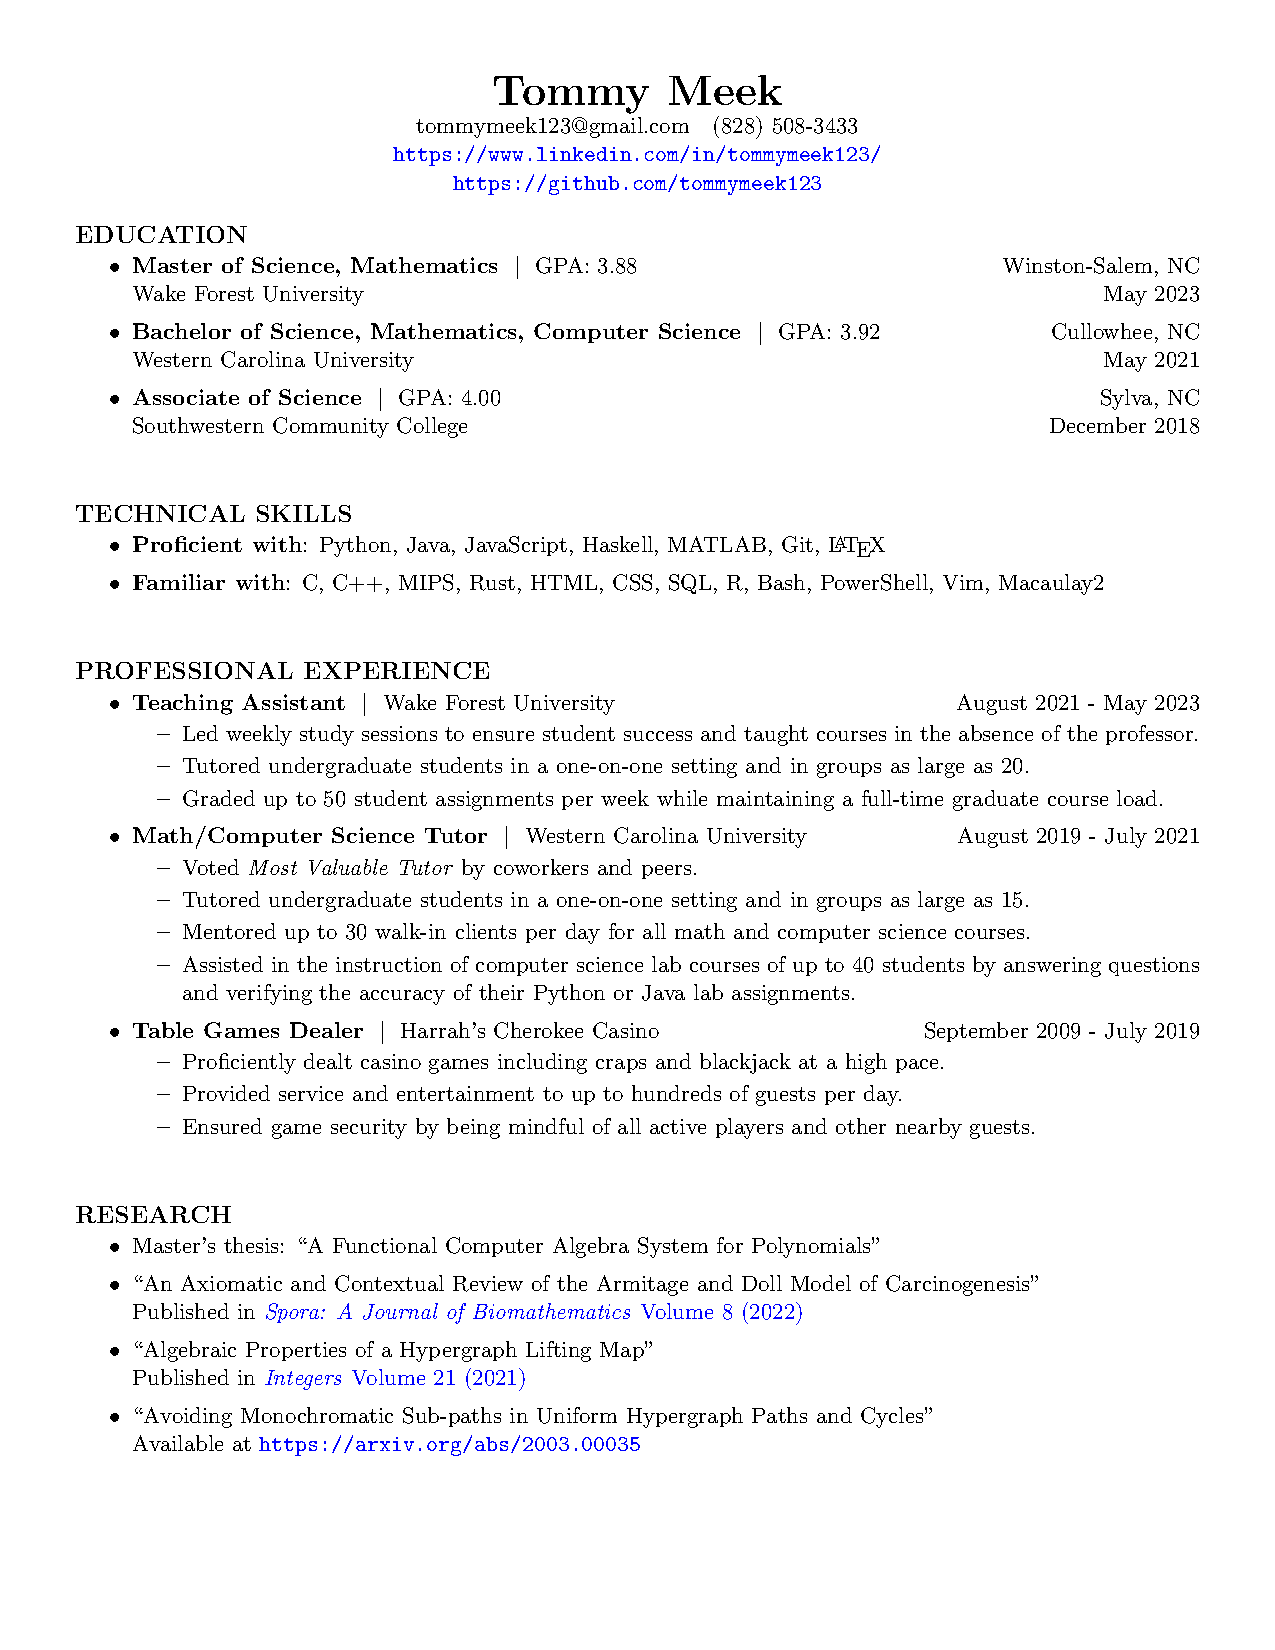
\includepdf[trim=-30mm 0mm -10mm 0mm, pages=-]{CV.pdf}

\end{document}